\documentclass[border=6pt]{standalone}
\usepackage{amsmath,bm,tikz}
\usetikzlibrary{arrows,positioning,patterns,shapes}
\pgfdeclarepatternformonly{stripes}
{\pgfpointorigin}{\pgfpoint{0.25cm}{0.25cm}}
{\pgfpoint{0.25cm}{0.25cm}}
{
    \pgfpathmoveto{\pgfpoint{0cm}{0cm}}
    \pgfpathlineto{\pgfpoint{0.25cm}{0.25cm}}
    \pgfpathlineto{\pgfpoint{0.25cm}{0.12cm}}
    \pgfpathlineto{\pgfpoint{0.12cm}{0cm}}
    \pgfpathclose%
    \pgfusepath{fill}
    \pgfpathmoveto{\pgfpoint{0cm}{0.12cm}}
    \pgfpathlineto{\pgfpoint{0cm}{0.25cm}}
    \pgfpathlineto{\pgfpoint{0.12cm}{0.25cm}}
    \pgfpathclose%
    \pgfusepath{fill}
}


\begin{document}
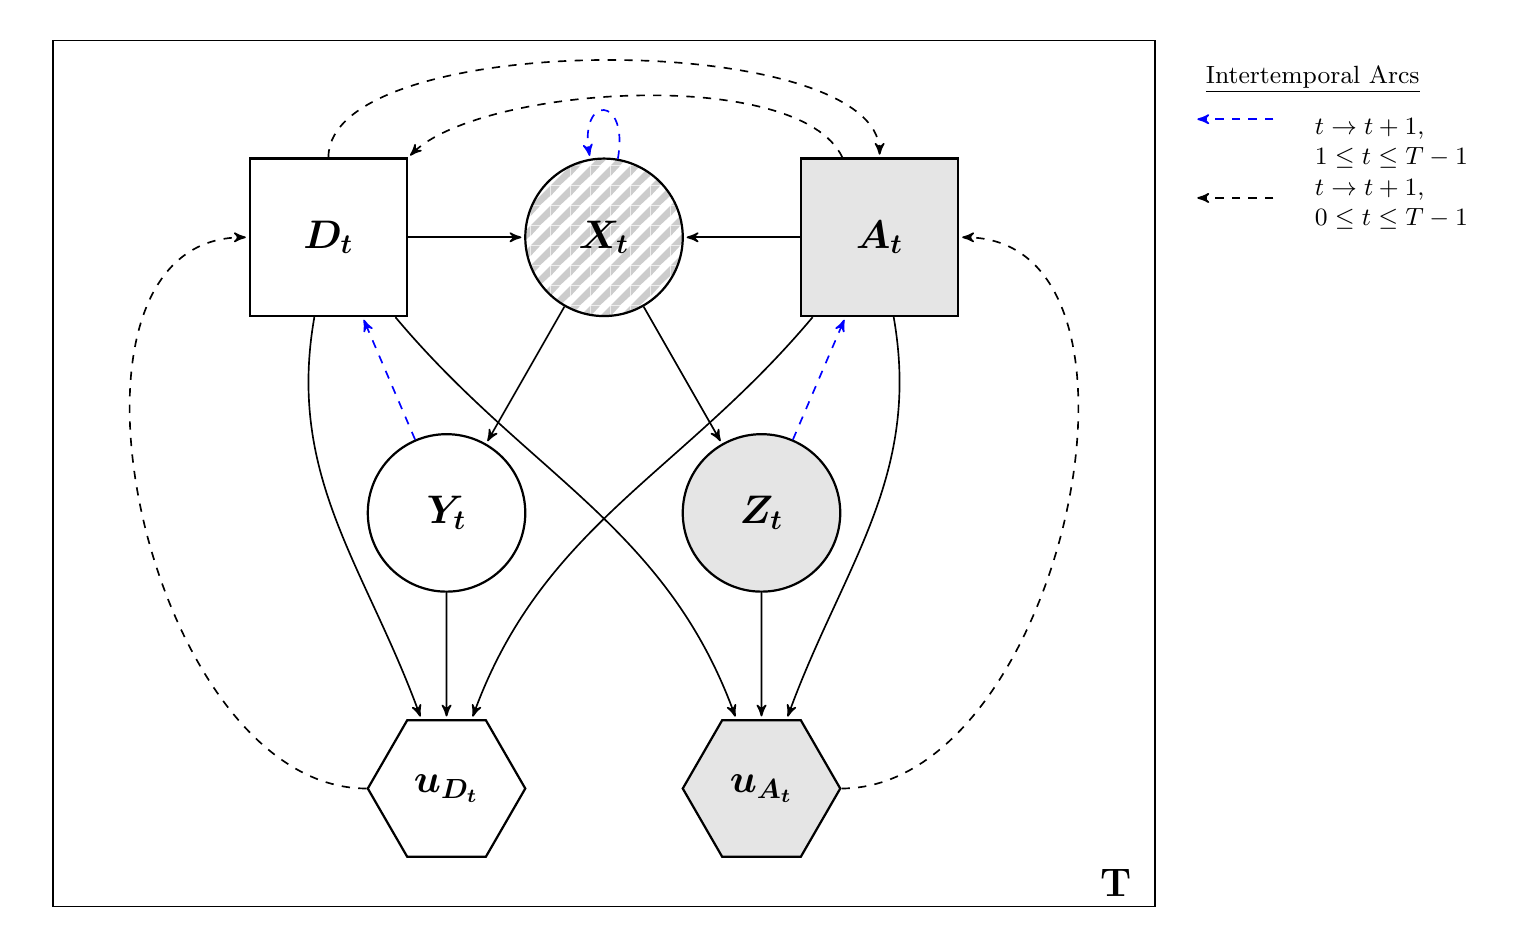
\begin{tikzpicture}[->,>=stealth',shorten >=1pt,auto,node distance=3.5cm,
                    semithick]
  \tikzstyle{uncertain}=[circle,pattern=stripes,
                                    pattern color=gray!40,
                                    thick,
                                    minimum size=2cm,
                                    draw=black,
                                    font=\Large]
  \tikzstyle{uncertainX}=[circle,thick,
                                    minimum size=2cm,
                                    draw=black,
                                    fill=gray!20,
                                    font=\Large]
  \tikzstyle{uncertainY}=[circle,thick,
                                    minimum size=2cm,
                                    draw=black,
                                    fill=white!20,
                                    font=\Large]
  \tikzstyle{Attacker_utility}=[regular polygon,regular polygon sides=6,
                                    thick,
                                    minimum size=2cm,
                                    draw=black,
                                    fill=gray!20,
                                    font=\Large]
  \tikzstyle{Defender_utility}=[regular polygon,regular polygon sides=6,
                                    thick,
                                    minimum size=2cm,
                                    draw=black,
                                    fill=white,
                                    font=\Large]
  \tikzstyle{Attacker_decision}=[rectangle,
                                    thick,
                                    minimum size=2cm,
                                    draw=black,
                                    fill=gray!20,
                                    font=\Large]
  \tikzstyle{Defender_decision}=[rectangle,
                                    thick,
                                    minimum size=2cm,
                                    draw=black,
                                    fill=white,
                                    font=\Large]
  \tikzstyle{texto}=[label]			
  \node[uncertain](D)   {$\bm{X_{t}}$};
  \node[Defender_decision] (A) [left of=D]  {$\bm{D_{t}}$};
  \node[Attacker_decision] (B) [right of=D] {$\bm{A_{t}}$};
  \node[uncertainY](YD)   [xshift = -2cm, yshift = 0.0cm, below of = D] {$\bm{Y_{t}}$};
  \node[uncertainX](YA)   [xshift = 2cm, yshift = 0.0cm,below of = D] {$\bm{Z_{t}}$};
  \node[Defender_utility]  (C) [below of=YD] {$\bm{u_{D_t}}$};
  \node[Attacker_utility]  (E) [below of=YA] {$\bm{u_{A_t}}$};
  \path (A) edge[out = 260, in =110]    node {} (C)
            edge[out = 310, in =110]    node {} (E)
            edge[]    node {} (D)
            %edge[out =270 , in =135]    node {} (YD)
        (B) edge[out = 280, in =70]    node {} (E)
            edge[out = 230, in =70]    node {} (C)
            edge[]    node {} (D)
            %edge[out =270 , in =45]    node {} (YA)
        %(D) edge    node {} (C)
           % edge    node {} (E)
        (D)   edge    node {} (YD)
            edge    node {} (YA)
        (C) edge[dashed, out=180, in=180,loop,looseness=1]    node {} (A) 
        (E) edge[dashed, out=0, in=0,loop,looseness=1]    node {} (B)
        (D) edge[dashed, blue, out=80, in=100,loop,looseness=6]    node {} (D)
        (YD) edge[dashed, blue]    node {} (A)
            edge[]    node {} (C)
        (YA)  edge[dashed, blue]    node {} (B)
             edge[]    node {} (E)
        (A) edge[dashed, out=90, in=90,loop,looseness=0.6]    node {} (B)
        (B) edge[dashed, out=115, in=45,loop,looseness=0.6]    node {} (A);
        %(A) edge[dashed, out=90, in=90,loop,looseness=0.5]    node {} (B)
        %(B) edge[dashed, out=135, in=45,loop,looseness=0.5]    node {} (A);


    \draw (-7,2.5) rectangle (7,-8.5);
    \node[draw=none] at (6.5, -8.2) {{\Large \textbf{T}}};
    %\node[draw=none] at (4.75, 0.5) {\footnotesize \begin{tabular}{c} $t \to t+1$, \\ $t<T$ \end{tabular}};
    %\node[draw=none] at (-4.75, 0.5) {\footnotesize \begin{tabular}{c} $t \to t+1$, \\ $t<T$ \end{tabular}};
    \node[draw=none] at (9, 2) {{\small \underline{Intertemporal Arcs}}};
    \draw [dashed, blue] (8.5, 1.5) -- (7.5,1.5);
    \draw [dashed] (8.5, 0.5) -- (7.5,0.5);
    \node[draw=none] at (10, 1) {\small \begin{tabular}{l} \\ $t \to t+1$,\\ $1\le t \le T-1$\\$t \to t+1$, \\ $0\le t \le T-1$ \end{tabular}};
\end{tikzpicture}
\end{document}
